\documentclass{article}
\usepackage{graphicx}

\usepackage{subfigure}
\usepackage{hyperref}
\usepackage{amsmath}

\usepackage{pifont}% http://ctan.org/pkg/pifont
\newcommand{\cmark}{\ding{51}}%
\newcommand{\xmark}{\ding{55}}%

\begin{document}

\title{Case Study: \textit{uniNDTotal} Consistency Relation}
%\author{Author's Name}

\maketitle

%\begin{abstract}
%The abstract text goes here.
%\end{abstract}

\section{Motivation and origin}

--

\section{Specification}
\label{sec:spec}

\subsection{Metamodels (\textit{M,N})}
\label{sec:metamodels}

\begin{figure}[ht]
    \centering
    \mbox{\subfigure[$M$]{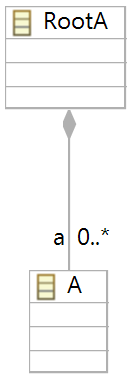
\includegraphics[scale=0.25]{printscreens/MMA.png}}\qquad\qquad
          \subfigure[$N$]{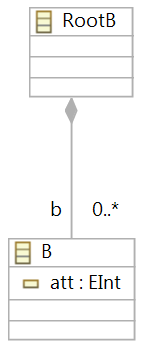
\includegraphics[scale=0.28]{printscreens/MMBatt.png}}
          }
    \caption{Metamodels}
    \label{fig:Meta}
\end{figure}


\subsection{Consistency relation (\textit{R})}
\label{sec:CR}

\textbf{Type:} \textit{uniNDTotal},  $one <> some$\\

For every $M$ instance there
exists \textbf{one} $N$ instance such that both are related by $R$;

For every $N$ instance there
exists \textbf{exactly one} $M$ instance such that both are related by $R$.

~\\

\begin{center}
\begin{tabular}{| c | c | c | c | c | }
  \hline                        
   & injective & entire & simple & surjective \\
  \hline 
  $R$ & \cmark & \cmark &  & \cmark\\
  \hline  
\end{tabular}
\end{center}


\textbf{Definition}\\

For every \textit{A} in \textit{RootA} there
exists \textbf{one} \textit{B} in \textit{RootB}; \footnote{This direction is non deterministic since any \textit{B} is consistent regardless of its attribute value.}

For every \textit{B} in \textit{RootB} there
exists \textbf{exactly one} \textit{A} in \textit{RootA}.


%------------------------------------
\pagebreak
\section{Test instances (\textit{m,n})}

\subsection{One A}
\label{sec:oneA}

\begin{figure}[ht]
    \centering
    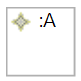
\includegraphics[scale=0.35]{printscreens/inst-oneA.png}
    \caption{One A ($m$)}
    \label{fig:oneA}
\end{figure}

\subsection{No As}
\label{sec:noAs}

\begin{center}
\textit{(no As ($m$))}
\end{center}

\subsection{One B attribute 0}
\label{sec:oneBatt0}

\begin{figure}[ht]
    \centering
    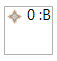
\includegraphics[scale=0.45]{printscreens/inst-oneBatt0.png}
    \caption{One B with attribute value 0 ($n$)}
    \label{fig:oneBatt0}
\end{figure}

\subsection{One B attribute 15}
\label{sec:oneBatt15}

\begin{figure}[ht]
    \centering
    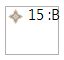
\includegraphics[scale=0.45]{printscreens/inst-oneBatt15.png}
    \caption{One B with attribute value 15 ($n$)}
    \label{fig:oneBatt15}
\end{figure}



%-------------------------------
\pagebreak

\subsection{Transformations to assess}
~\\
\begin{center}
\begin{tabular}{| c | c | c | c | c | }
  \hline                        
   & $m$ & $n$ & $\overrightarrow{R}$ & $\overleftarrow{R}$ \\
  \hline 
  T1 & \nameref{sec:oneA} & \nameref{sec:oneBatt0} & \cmark & \\
  \hline
  T2 & \nameref{sec:noAs} & \nameref{sec:oneBatt15} &  & \cmark\\
  \hline
  T3 & \nameref{sec:oneA} & \nameref{sec:oneBatt15} & \cmark & \\
  \hline
\end{tabular}
\end{center}
~\\

%------------------------------------
\pagebreak
\section{Tools assessment}

\subsection{\textit{eMoflon}}

\subsubsection{Specification implementation}

\textit{Specification environment}: Enterprise Architect~\cite{EA}
~\\

\textbf{Metamodels}

\begin{figure}[ht]
    \centering
    \mbox{\subfigure[$M$]{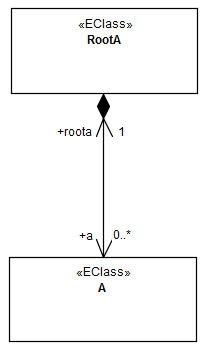
\includegraphics[scale=0.45]{printscreens/ea-MMA.png}}\quad
          \subfigure[$N$]{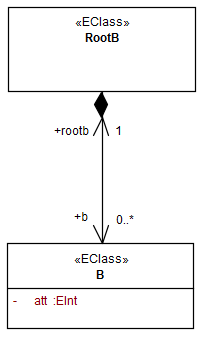
\includegraphics[scale=0.46]{printscreens/ea-MMBatt.png}}
          }
    \caption{Metamodels modelled as \textit{EA Ecore Diagrams}}
    \label{fig:eMoIMP1}
\end{figure}

~\\
\textbf{Consistency Relation}

\begin{figure}[ht]
  \centering 
  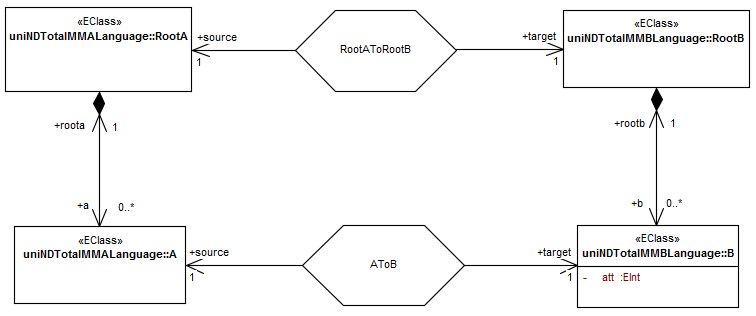
\includegraphics[scale=0.4]{printscreens/ea-MMAToMMBatt.png}
  \caption{\textit{TGG Schema Diagram}}
  \label{fig:bij-schema}
\end{figure}

\pagebreak

\begin{figure}[ht]
  \centering 
  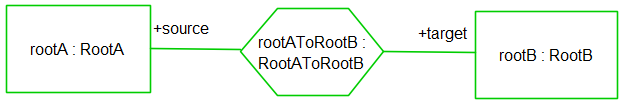
\includegraphics[scale=0.5]{printscreens/ea-RootAToRootB-rule.png}
  \caption{\textit{TGG Rule Diagram} RootAToRootB}
  \label{fig:ea-RootAToRootB-rule}
\end{figure}

~\\

\begin{figure}[ht]
  \centering 
  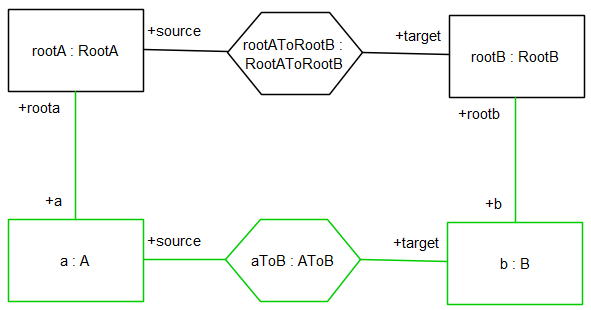
\includegraphics[scale=0.5]{printscreens/ea-AToB-rule.png}
  \caption{\textit{TGG Rule Diagram} AToB}
  \label{fig:ea-AToB-rule}
\end{figure}

%-------------------------------------------------

\subsubsection{Instances transformation results}

\textit{Integration environment}: Eclipse Modelling Tools~\cite{EMT}

~\\

%  \hline                        
%   & $m$ & $n$ & $\overrightarrow{R}$ & $\overleftarrow{R}$ \\
%  \hline 
%  T1 & \nameref{sec:oneA} & \nameref{sec:oneBatt0} & \cmark & \\
%  \hline
%  T2 & \nameref{sec:noAs} & \nameref{sec:oneBatt15} &  & \cmark\\
%  \hline
%  T3 & \nameref{sec:oneA} & \nameref{sec:oneBatt15} & \cmark & \\
%  \hline
T1 - \nameref{sec:oneA} / \nameref{sec:oneBatt0} ($\overrightarrow{R}$)
\begin{figure}[ht]
    \centering
    \mbox{\subfigure[$m$]{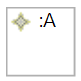
\includegraphics[scale=0.35]{printscreens/inst-oneA.png}}\quad\qquad
          \subfigure[$n$]{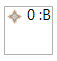
\includegraphics[scale=0.45]{printscreens/inst-oneBatt0.png}}
          }
    \caption{T1 result}
    \label{fig:T1}
\end{figure}

\pagebreak

T2 - \nameref{sec:noAs} / \nameref{sec:oneBatt15} ($\overleftarrow{R}$)
\begin{figure}[ht]
    \centering
    \mbox{\subfigure[$m$]{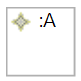
\includegraphics[scale=0.35]{printscreens/inst-oneA.png}}\quad\qquad\quad
          \subfigure[$n$]{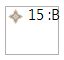
\includegraphics[scale=0.45]{printscreens/inst-oneBatt15.png}}
          }
    \caption{T2 result}
    \label{fig:T2}
\end{figure}

~\\

T3 - \nameref{sec:oneA} / \nameref{sec:oneBatt15} ($\overrightarrow{R}$)
\begin{figure}[ht]
    \centering
    \mbox{\subfigure[$m$]{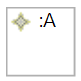
\includegraphics[scale=0.35]{printscreens/inst-oneA.png}}\quad\qquad\quad
          \subfigure[$n$]{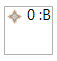
\includegraphics[scale=0.45]{printscreens/inst-oneBatt0.png}}
          }
    \caption{T3 result}
    \label{fig:T3}
\end{figure}

~\\

\subsubsection{Assessment}



\begin{center}
\begin{tabular}{| r | c | }
  \hline                        
  correct & \cmark \\
  \hline
  hippocratic &  \\
  \hline 
  undoable &  \\
  \hline 
  history-ignorant &  \\
  \hline 
  simply-matching &  \\
  \hline 
  matching &  \\
  \hline 
  least-change &  \\
  \hline   
\end{tabular}
\end{center}


%------------------------------------
\pagebreak
\subsection{\textit{Echo}}
\subsubsection{Specification implementation}
\textit{Specification environment}:
~\\

\textbf{Metamodels}
~\\

\textbf{Consistency Relation}


\subsubsection{Instances transformation results}
\textit{Integration environment}:
~\\



\subsubsection{Assessment}

\begin{center}
\begin{tabular}{| r | c |}
  \hline                        
  correct & \\
  \hline
  hippocratic & \\
  \hline 
  undoable & \\
  \hline 
  history-ignorant & \\
  \hline 
  simply-matching & \\
  \hline 
  matching & \\
  \hline 
  least-change & \\
  \hline   
\end{tabular}
\end{center}

%------------------------------------
\pagebreak
\subsection{\textit{Focal}}
\subsubsection{Specification implementation}
\textit{Specification environment}:
~\\

\textbf{Metamodels}
~\\

\textbf{Consistency Relation}
\subsubsection{Instances transformation results}
\textit{Integration environment}:
~\\


\subsubsection{Assessment}

\begin{center}
\begin{tabular}{| r | c |}
  \hline                        
  correct & \\
  \hline
  hippocratic & \\
  \hline 
  undoable & \\
  \hline 
  history-ignorant & \\
  \hline 
  simply-matching & \\
  \hline 
  matching & \\
  \hline 
  least-change & \\
  \hline   
\end{tabular}
\end{center}
%-------------------------------------
\pagebreak
\subsection{Summary table and comparison}

\pagebreak
\section{Discussion}

\pagebreak
\begin{thebibliography}{1}

\bibitem{Perdita}http://homepages.inf.ed.ac.uk/perdita/ 

\bibitem{Perdita2}Stevens, Perdita. "Bidirectional model transformations in QVT: Semantic issues and open questions." Model Driven Engineering Languages and Systems. Springer Berlin Heidelberg, 2007. 1-15.

\bibitem{Perdita3}Stevens, Perdita. "Observations relating to the equivalences induced on model sets by bidirectional transformations." Electronic Communications of the EASST 49 (2012).

%------------------

\bibitem{EA}http://www.sparxsystems.com/products/ea/index.html

\bibitem{EMT}http://www.eclipse.org/


\end{thebibliography}



\end{document}